\section{效果演示说明}
% 这部分计划写的内容:
% - 附上效果图
% - 如何操作(例如先按 reset 再按 start 可以随机产生初始棋局和先手玩家)

\subsection{实验板使用}\label{subsection:circuit-usage}
\begin{figure}[H]
    \centering
    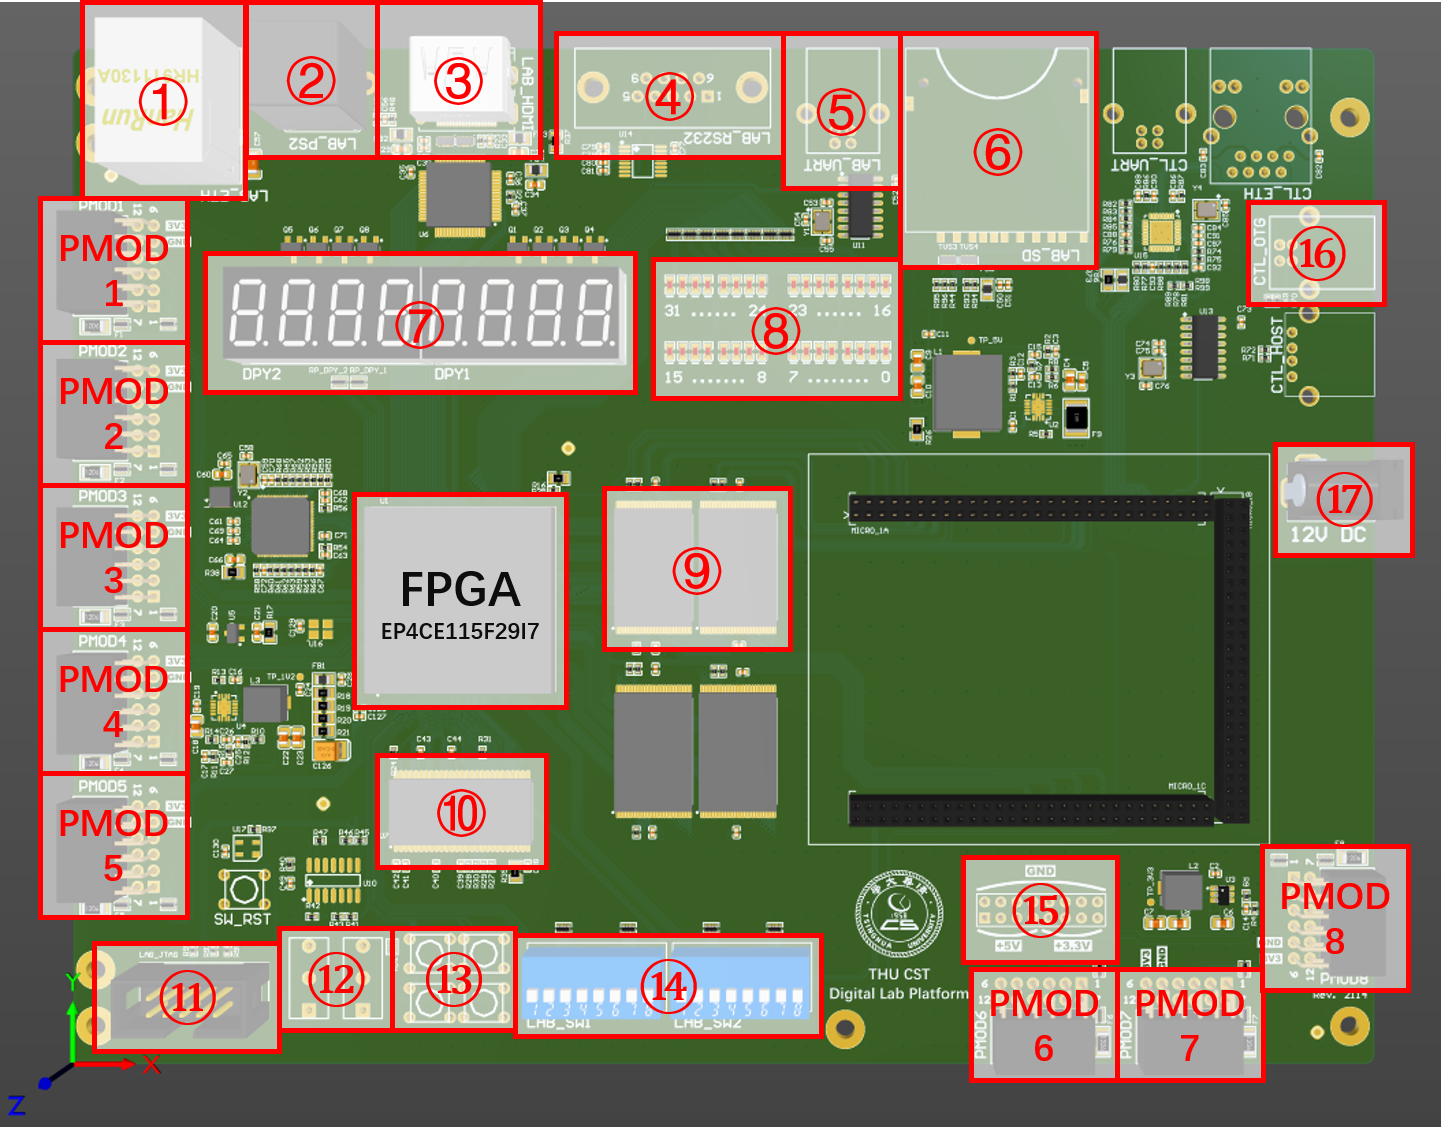
\includegraphics[scale=0.50]{images/board_anno.png}
    \caption{课程提供的实验板}
    \label{fig:board_anno}
\end{figure}

本项目在所给实验板上实现。使用的接口包括:
\begin{itemize}
    \item \textcircled{2}:PS/2接口,连接键盘;
    \item \textcircled{3}:HDMI接口,连接显示器;
    \item \textcircled{11}:FPGA JTAG调试接口,连接USB blaster,并接入电脑;
    \item \textcircled{12}去抖按键:用于开始游戏,生成随机初始棋局和随机先手玩家;
    \item \textcircled{17}电源:接入 12V 直流电源,用于给实验板供电。
\end{itemize}

\subsection{运行游戏}
在依第 \ref{subsection:circuit-usage} 节 连接好接口后,或者在需要重新开始一局游戏时,先按下“去抖按键”的左键(下称 reset 按钮),然后按下“去抖按键”的右键(下称 start 按钮),即可产生随机初始棋局和随机先手玩家,并自动开始游戏。

游戏开始后,玩家按第 \ref{subsubsection:operate-rules} 节(操作规则)所述方法进行操作。

\subsection{效果演示}

游戏效果演示视频见网络学堂提交的压缩包下的 \verb|doc/Videos| 文件夹。
\begin{figure}[H]
    \centering
    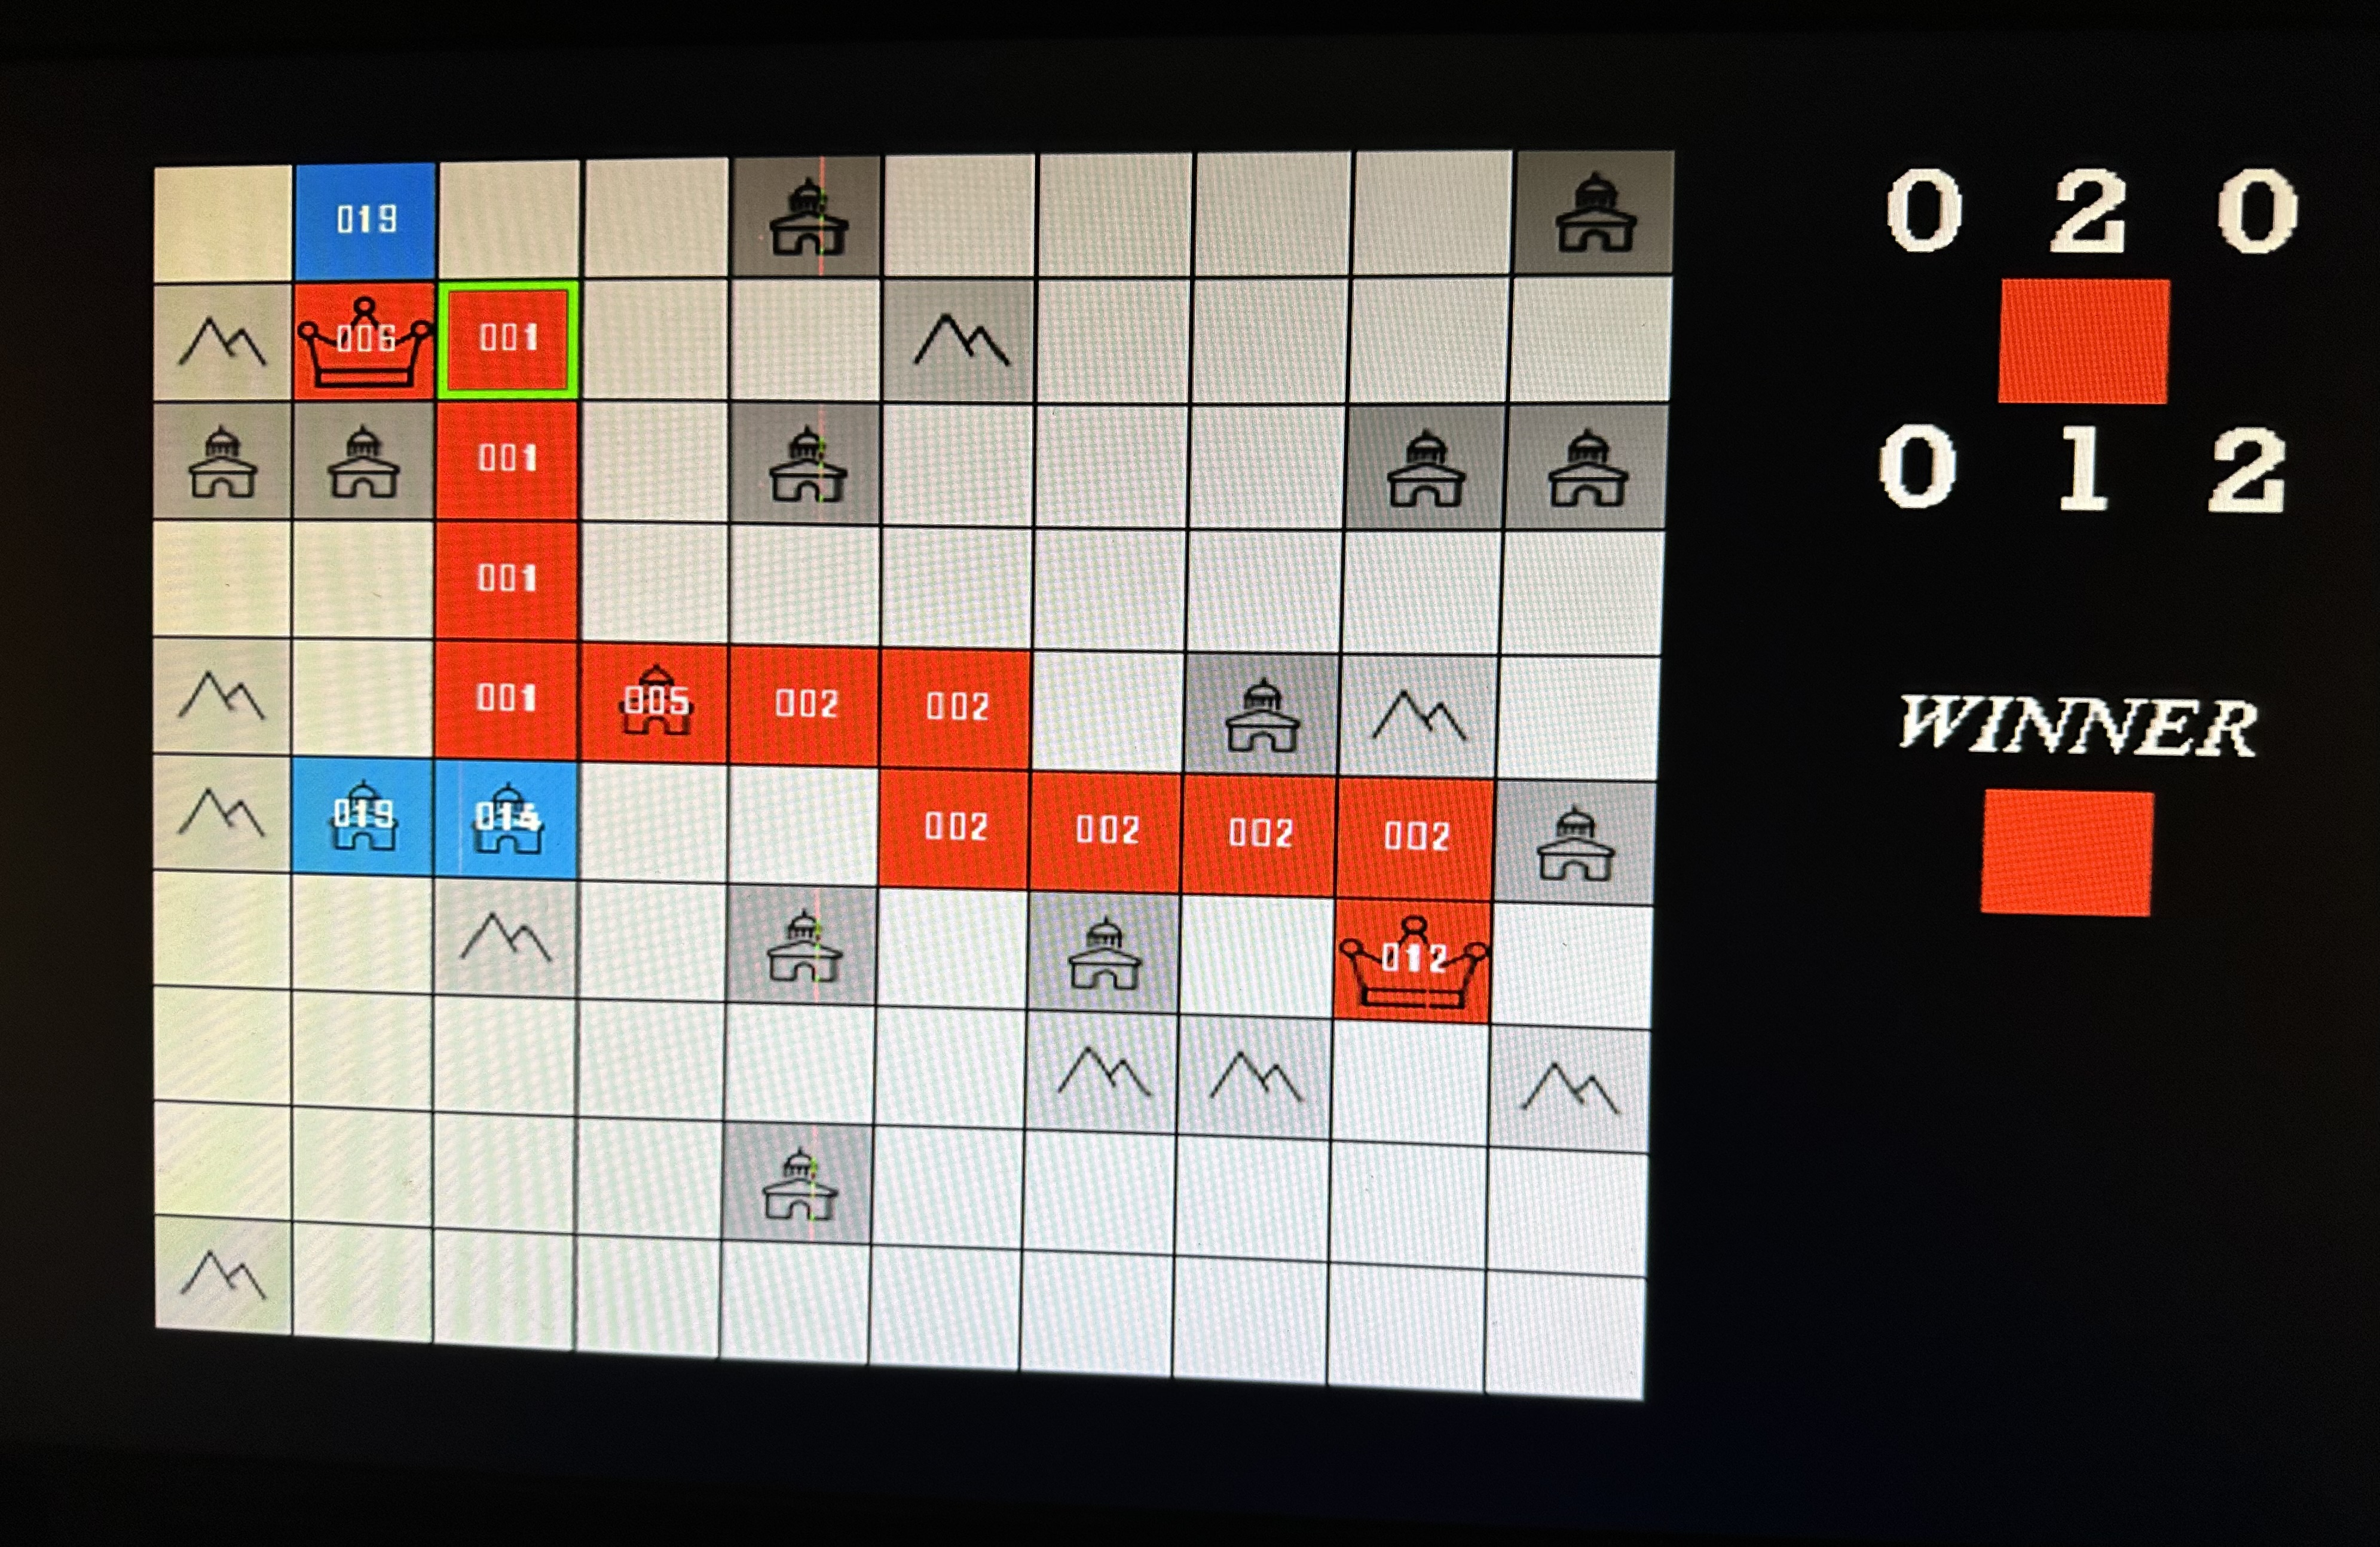
\includegraphics[scale=0.40]{images/demo.jpg}
    \caption{效果示例(红方胜利)}
    \label{fig:demo}
\end{figure}